% use paper, or submit
% use 11 pt (preferred), 12 pt, or 10 pt only

\documentclass[letterpaper, preprint, paper,11pt]{AAS}	% for preprint proceedings
%\documentclass[letterpaper, paper,11pt]{AAS}		% for final proceedings (20-page limit)
%\documentclass[letterpaper, paper,12pt]{AAS}		% for final proceedings (20-page limit)
%\documentclass[letterpaper, paper,10pt]{AAS}		% for final proceedings (20-page limit)
%\documentclass[letterpaper, submit]{AAS}			% to submit to JAS

\usepackage{bm}
\usepackage{amsmath}
\usepackage{subfigure}
%\usepackage[notref,notcite]{showkeys}  % use this to temporarily show labels
\usepackage[colorlinks=true, pdfstartview=FitV, linkcolor=black, citecolor= black, urlcolor= black]{hyperref}
\usepackage{overcite}
\usepackage{footnpag}			      	% make footnote symbols restart on each page
\usepackage{float}



\PaperNumber{XX-XXX}



\begin{document}

\title{\textsf{\textbf{Induced Fragmentation of Asteroids during Close Encounters}}}
\author{\textsf{Bryan Tester}\thanks{PhD student at University of Strathclyde, United Kingdom}
\ and \textsf{Prof. Massimiliano Vasile}\thanks{Professor at University of Strathclyde, United Kingdom}}

\maketitle{} 		


\begin{abstract}
We consider the behaviour of rotating binary asteroids as they pass through Earth's Hill sphere, with primary interest in the effect the tidal force has on the interaction between the two components of the binary and their post-encounter trajectories. We focus on contact binary asteroids bound by a regolith bridge, using both direct numerical simulation and an analytical approach.
\end{abstract}

\section{Introduction}
Radar observations suggest that a significant portion of Asteroids with Earth-crossing orbits are binary systems, consisting of two components in contact with or in close proximity to each other. As shown by work such as that of Farinella \textit{et al} \cite{binaryevo} in the early 1990s, gravitational encounters can significantly alter the orbits and integrity of binary asteroids. Clearly it is important to be able to accurately predict the motion of these bodies to give maximum warning of any possible Earth collision event. The work presented here is inspired by that of Borum \textit{et al}\cite{exchange}. In our work we revisit some of the previously discussed cases and then expand to include “Contact Binaries” (single asteroids formed primarily by two large boulders); we consider both gravitationally bound pairs and those bound by a regolith bridge, as illustrated in Figure ~\ref{fig:Pic} (this mechanism is similar to that discussed by Sanchez \& Scheeres \cite{dustbound}). We also model an attempted deflection of the asteroid prior to the close encounter. Our analysis has been performed using both numerical simulations and by taking an analytical approach.
\begin{figure}[H]
\centering
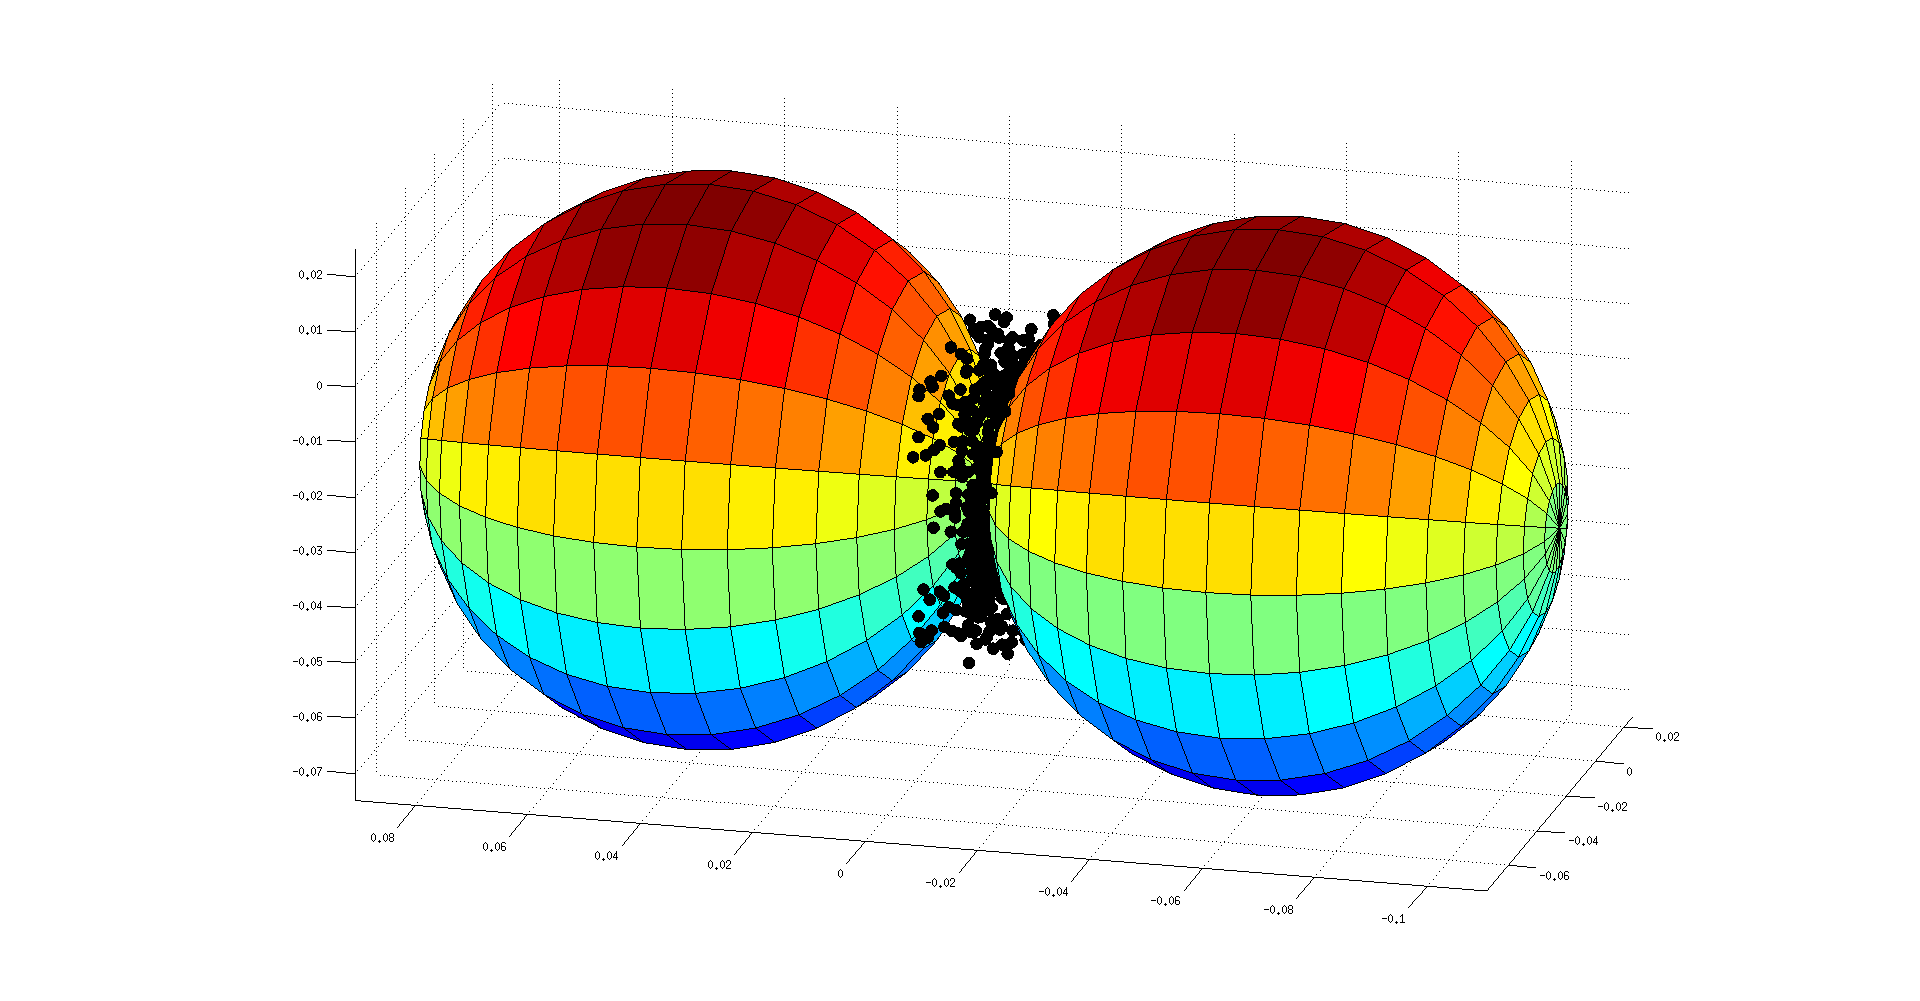
\includegraphics[width=0.6\textwidth]{binary_3d.eps} 
\caption{Simulation of two 10 cm diameter spheres joined by a finer regolith bridge.} 
\label{fig:Pic}
\end{figure} 


\section{Equations of Motion}
The analytical approach to characterising the system is based upon the full equations of motion in a rotating reference frame, with the rotation of the reference frame such that the barycentre of the system remains at a constant angle to the Earth. The resulting equations can be split into two separate parts, detailing the motion of the barycentre and the relative motion of the binary components respectively. For obvious complexity reasons we choose to neglect the individual effect of the particles in the regolith bridge but opt instead to incorporate their net effect on the force between the main binary components into a single term. Figure ~\ref{fig:Analy} shows the break-up time predicted by the analytical approach for an example binary pair during a close encounter, compared to the actual break-up seen in numerical simulations; the break-up is observed as the energy trace transitions from the oscillating regime to a steady state.
\begin{figure}[H]
\centering
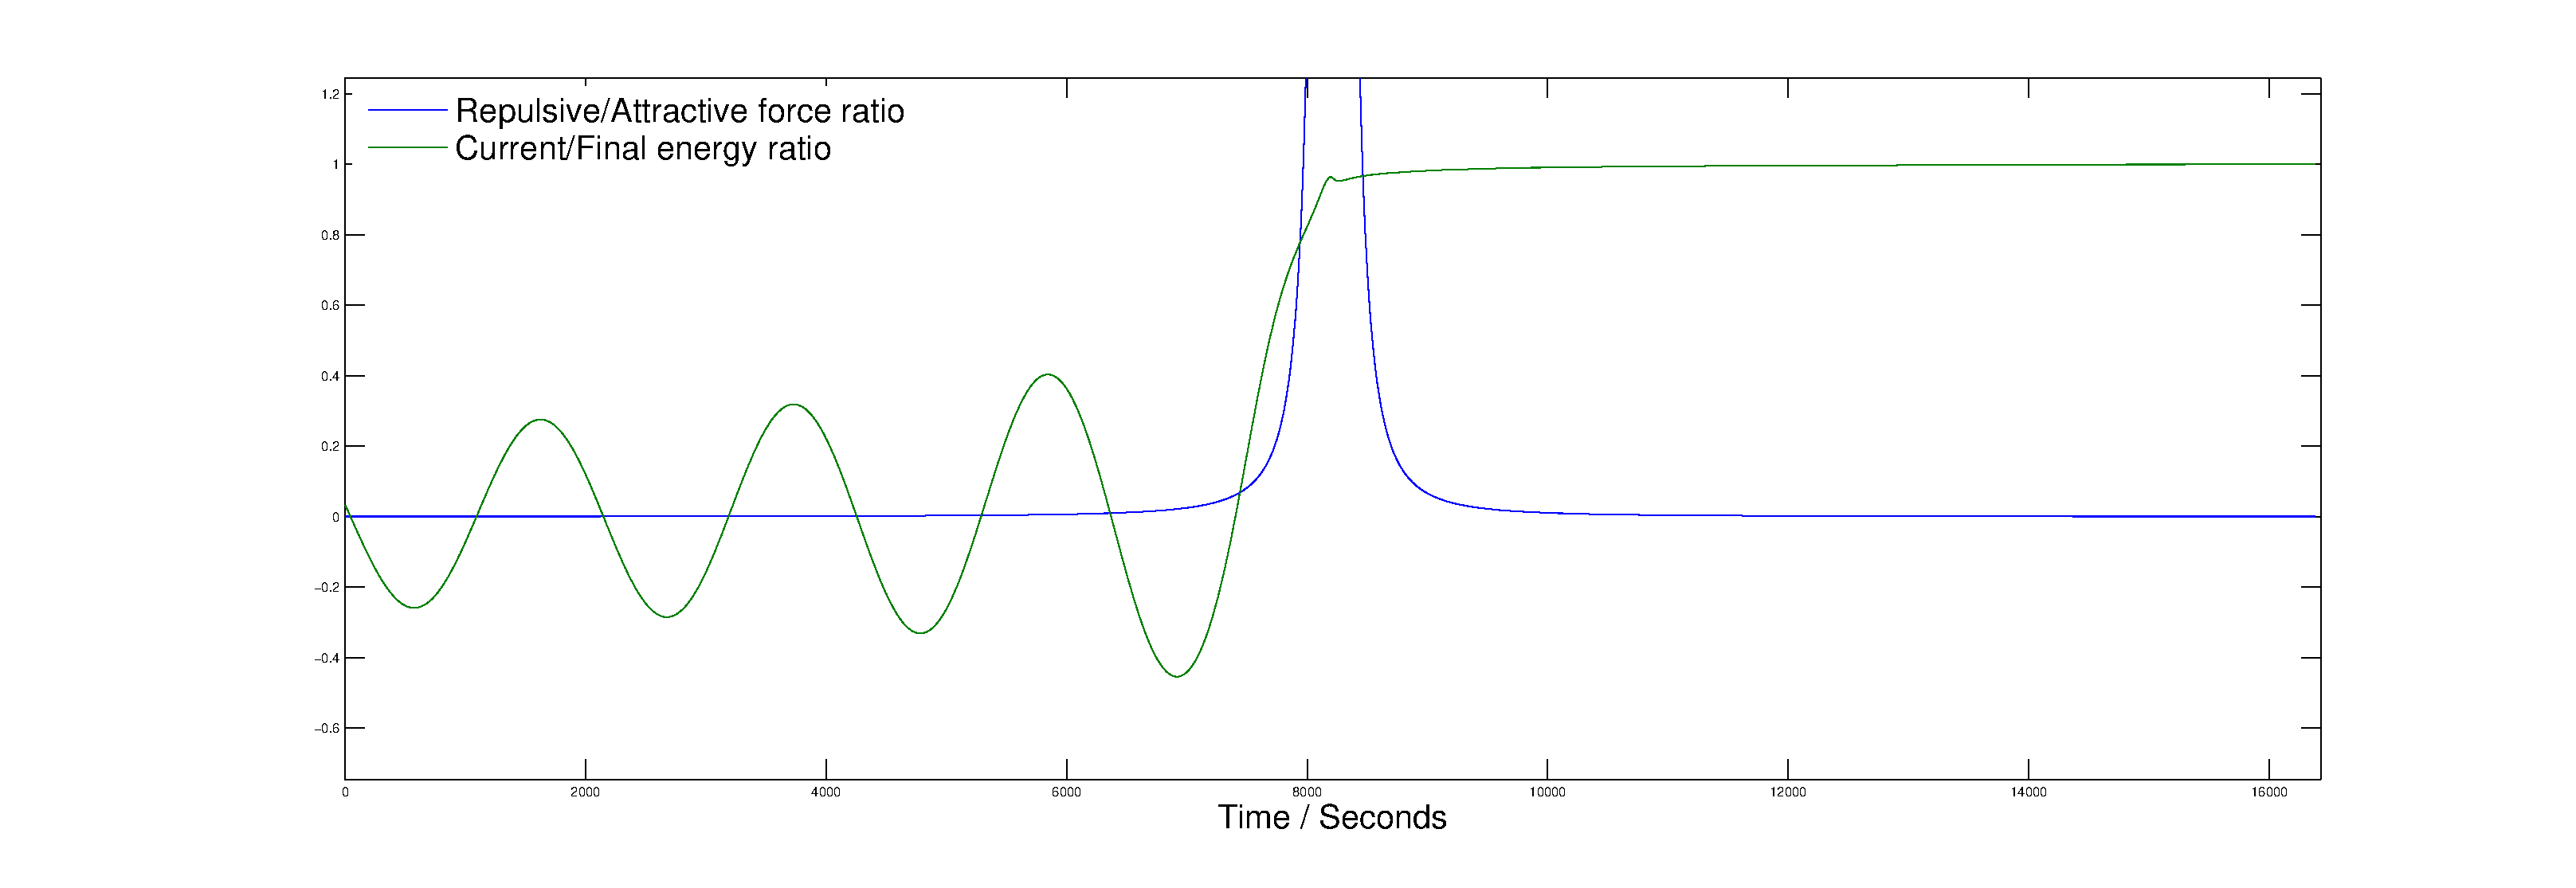
\includegraphics[width=1.2\textwidth]{binary_analy.eps} 
\caption{Plots of the ratio between attractive and repulsive forces predicted by analytical model and Gravitational potential and kinetic energy of 1 component of the binary as a fraction of its final energy state from numerical simulations.} 
\label{fig:Analy}
\end{figure} 

\section{Numerical Simulations}
The numerical simulations are run using a custom multi-body code, which includes full inter-particle gravitational interactions, London dispersion forces and Soft-Body collisions similar to those implemented in \textit{PKDGRAV} by Schwartz \textit{et al}\cite{soft}.
Previous work considering the orbits of binary and rubble pile asteroid has only considered gravitational interactions between the components. We consider encounters with a range of Earth-Asteroid two-body energies and varying binary asteroid rotation speeds; the binary components are placed in a mutual circular orbit in each case with the force between them artificially varied to simulate the effects of a regolith bridge binding the two components.
\begin{figure}[H]
\centering
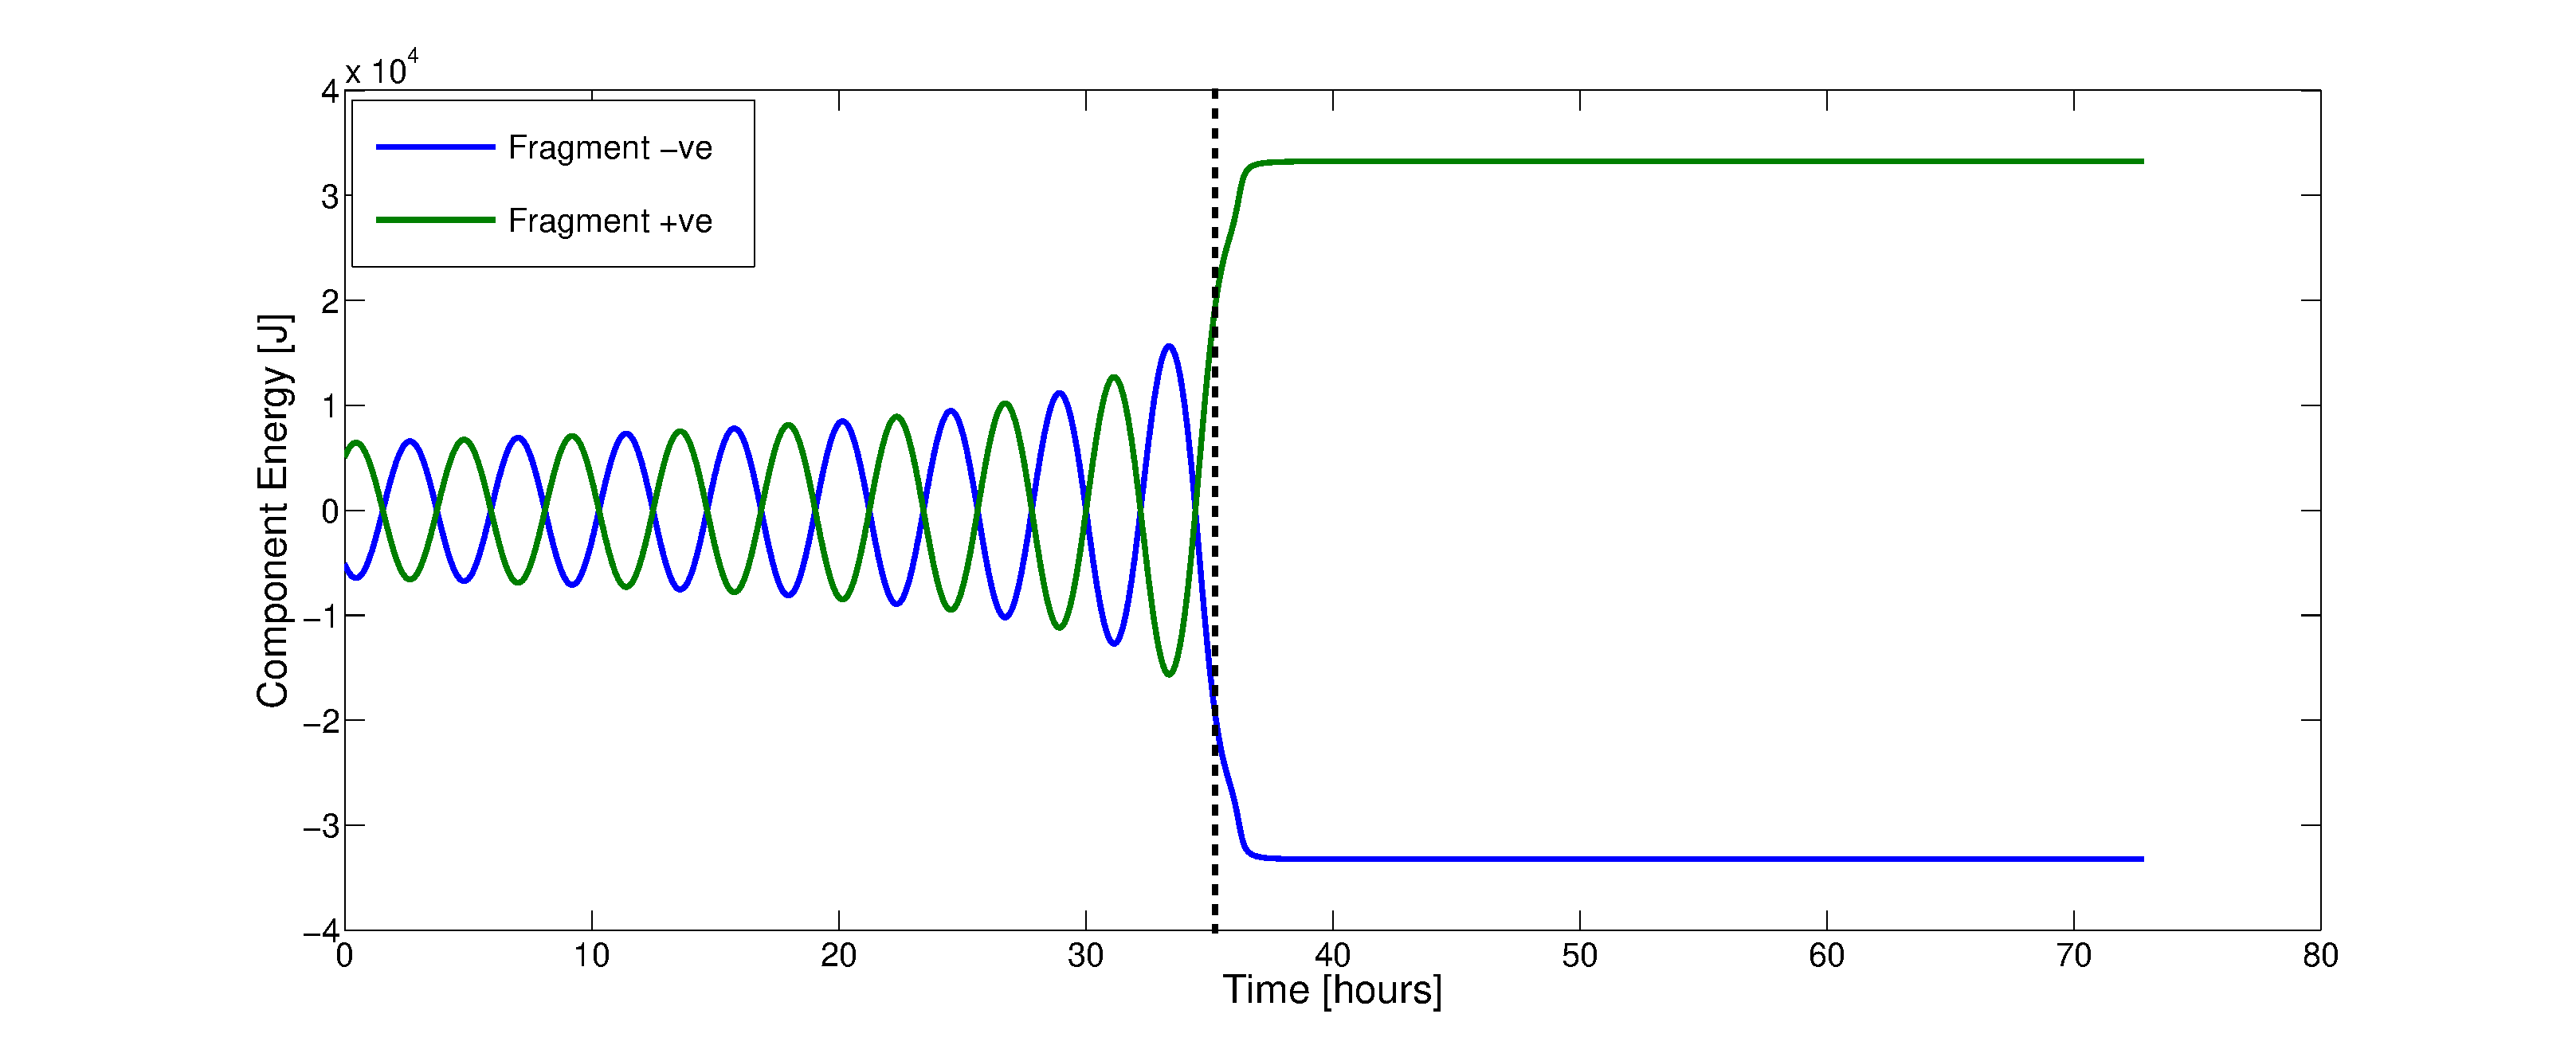
\includegraphics[width=1.2\textwidth]{binary_num.eps} 
\caption{Plots of the Gravitational potential and kinetic energy of both components of the binary from numerical simulations.} 
\label{fig:Num}
\end{figure}
 Figure ~\ref{fig:Num} shows the output of such a simulation for a binary on a Parabolic trajectory; after the fragmentation one components is "captured" (having its orbital energy reduced below zero) and the other escapes (gaining orbital energy).  
Full numerical simulations of two boulders bound by such a regolith bridge on a Hyperbolic trajectory are also performed and the effect of the tidal forces on the integrity of the bridge is investigated.


\section{Conclusion}
We present a methodology to model contact binary asteroids bound by regolith during an encounter with a large body such as Earth. Any conclusions drawn from this research will allow for enhanced accuracy in the prediction of asteroid trajectories and allow for better planning in any mission to capture or deflect such an object.

\bibliographystyle{AAS_publication}   % Number the references.
\bibliography{references_me}   % Use references.bib to resolve the labels.



\end{document}
